\graphicspath{{chapt_dutch/}{intro/}{chapt2/}{chapt3/}{chapt4/}{chapt5/}{chapt6/}{chapt7/}{chapt8/}}

% Header
\renewcommand\evenpagerightmark{{\scshape\small Chapter 4}}
\renewcommand\oddpageleftmark{{\scshape\small Detector Control System for RPCs at GIF++}}

\renewcommand{\bibname}{References}

\hyphenation{}

\chapter[Detector control system for RPCs at GIF++]%
{Detector control system for RPCs at GIF++}\label{chapt:4}
This chapter summarizes the High Luminosity LHC (HL-LHC) program and the setup of the Gamma Irradiation Facility (GIF++), where the already-installed and future detectors are being tested. It further briefly explains the WinCC-OA program and the detector control system for the CMS RPCs project at the GIF++. The last section is devoted to the RPC performance study at the GIF++ setup. The work described in this chapter is documented in the publication~\cite{1748-0221-11-10-C10013}.  
\section{The HL-LHC program and the CMS detector upgrade}
The physics program using the Large Hadron Collider (LHC) began in 2009 at low energy (1.18\,TeV per beam), which has increased gradually to 7 and 8\,TeV in the following years. The two-year duration is termed as Run-I with a total delivered integrated luminosity of around 30\,fb$^{-1}$ for its major experiments, CMS and ATLAS, at 50\,ns bunch spacing with peak instantaneously luminosity being 7$\times 10^{33}\text{cm}^{-2}\text{s}^{-1}$. The highlight of  Run-I has been the observation of the Higgs boson that lead the high-energy physics community to foresee a challenging upgrade of the accelerator, known as the High Luminosity LHC (HL-LHC). After successful operation of Run-I, LHC was long shut down (LS1) for a two-year period (2013–14) in order to increase the centre-of-mass energy to near its nominal value. In the next LS2 period’s (2019–20) phase-I upgrade, the injector chain will be improved and upgraded to deliver extremely bright bunches (high intensity and low emittance) into the LHC. In LS3 (2023–26), with some basic changes during LS2, the LHC itself will be upgraded with new HL-LHC conditions. 

After LS1, the LHC started Run-II in 2015 at a record centre-of-mass energy of 13\,TeV with bunch spacing of 50\,ns, decreased to 25\,ns in 2016. The LHC successfully run for two years (2016–17) and delivered about 80\,fb$^{-1}$ physics data and is expected to deliver more than 100\,fb$^{-1}$ physics data with nominal instantaneous luminosity being 5$\times 10^{33}\text{cm}^{-2}\text{s}^{-1}$ at the end of Run-II. Run-III will last for about three years (2021–23) with an anticipated integrated luminosity of 300\,fb$^{-1}$.

HL-LHC is foreseen to begin operations around 2026, following the so-called ``Phase-II” machine upgrade at designed centre-of-mass energy $\sqrt{s}$ = 14\,TeV proton-proton collisions with instantaneous luminosities of between 5–7$\times 10^{34}\text{cm}^{-2}\text{s}^{-1}$ and expected 140 pile-up events on average. An integrated luminosity of 3\,ab$^{-1}$ is expected to be delivered during the ten-year run. This unprecedentedly large dataset will facilitate a wide spectrum of physics analyses, sensitive to high statistics, from precision tests of the Standard Model to New Physics searches with significantly enhanced discovery potential~\cite{1742-6596-515-1-012012}. An overview of the LHC and HL-LHC schedule is shown in Fig.~\ref{fig:hl_lhc_program}. 
 \begin{figure}[h]
\centering
\includegraphics[scale=0.52]{fig/lhc/HL-LHC-plan-2016-Plan-1}
\caption{\label{fig:hl_lhc_program} The LHC schedule summary and HL-LHC baseline plan with centre-of-mass energy in the upper thick-red line and the instantaneous luminosity lower red-thin line. Run-I started in 2011 at 7\,TeV subsequently increased to 8\,TeV in 2012, delivered up to 30\,fb$^{-1}$ in the two years. It was followed by a long shut down for two years (2013–14), upgraded to 13\,TeV centre-of-mass energy and finally Run-II started in 2015 and will end in 2018 delivering more than 100\,fb$^{-1}$ data, which will be followed by LS2 for two years. Run-III will span for three years (2021-23) at the designed centre-of-mass, 14\,TeV, with anticipated integrated luminosity of 300\,fb$^{-1}$. The HL-LHC program will start from 2024 with three years detectors up-gradation (LS3) followed by ten years Run-IV and Run-V. The instantaneous luminosity is expected to increase up to 5-7 times the nominal value at 14\,TeV centre-of-mass energy with expected total integrated luminosity of 3\,ab$^{-1}$~\cite{hl_lhc_industry}.}
\end{figure} 

The HL-LHC conditions will be achieved using novel cutting-edge technology. As the first step, the inner triplet quadrupole magnets in the insertion regions will be replaced with advanced and more radiation tolerant ones based on $\text{Nb}_{3}\text{Sn}$ superconducting technology. To effectively collide the proton beams head on, special superconducting radiofrequency crab cavities will be installed in the interaction regions to rotate both beams longitudinally with half of the crossing angle. Further HL-LHC improvements are: new technology and physical processes for beam collimation and 300-metre-long high-power superconducting links with negligible energy dissipation~\cite{Apollinari:2116337}. 

The high radiation environment at the HL-LHC will also introduce challenges to the installed detectors. Therefore, it is planned to perform upgrades of several sub-detectors of the CMS to maintain the excellent performance of the Phase-I detector under challenging HL-LHC conditions. A short description of the upgrades of the CMS sub-detectors is listed here.
\begin{itemize}
\item{\textbf{Tracker:}}
is installed near the interaction point and received a higher radiation dose. For HL-LHC, the tracker must have higher radiation tolerance to be able to operate efficiently up to an integrated luminosity of 3000\,fb$^{-1}$. Other properties are increased granularity to incorporate high pile-up events, improved two-track separation produced by high energy jets, reduced material in the tracking volume, robust pattern recognition, compliance with the L1 trigger upgrade, and extended tracking acceptance.
\item{\textbf{Barrel calorimeters:}}
As compared to endcaps, the barrel region is not under severe pressure from high radiation. However, in order to maintain exactly the same physics performance, the FE electronics of both sub-detectors (ECAL and HCAL) must be improved to satisfy the new L1 trigger requirements.
\item{\textbf{Endcap calorimeters:}}
will suffer significant radiation damage during the LH-LHC conditions and needs a re-examination of the ability of the detector’s active material and electronics to meet the requirements of 3000\,fb$^{-1}$.
\item{\textbf{Muon detectors:}}
It is important for Phase-II physics to keep the efficiency of the L1 muon triggers high, while maintaining $p_T$ thresholds low enough to collect a large fraction of Higgs, top quark, and electroweak bosons for conducting more sophisticated analysis. During Run-I and Run-II, no significant deterioration of key chamber parameters has been observed. Therefore, it is expected that the chambers themselves will provide excellent performance throughout the HL-LHC program. Some developments are instead foreseen for the FE electronics in the case of the DTs and the CSCs, which will be replaced with improved versions to increase radiation tolerance, readout speed and performance.

In the very forward regions, muon measurement can be made more efficient if a sufficient number of detector hits is measured for each muon track particular in the small regions not instrumented by the other muon sub-systems – CSC. It will enhance the redundancy of the muon system and enable obtaining a robust track reconstruction, including rejection of wrongly reconstructed tracks already at the Level-1 trigger. The two endcap regions suffer from high-muon and background rates as well as reduced magnetic bending. The Phase-II muon detector upgrade must recover an effective muon system in the forward region by adding new forward muon detectors, GE1/1 and GE2/1, equipped with Gaseous Electron Multiplier (GEM) detectors and RE3/1 and RE4/1 with improved RPC (iRPC) detectors see Fig.~\ref{fig:rpc_dt}, covering the pseudorapidity range up to 2.4. The ME0 chambers, also using GEM technology, extend the acceptance of the muon system further to $\abs{\eta} = 2.8$, by providing hits for triggering and for offline muon reconstruction~\cite{Collaboration:2283189}.

For RPC detectors, two important upgrades are planned – the RPC off-detector electronics (called link system) will be replaced and the RPC spatial coverage will be extended up to $\abs{\eta} = 2.4$ by installing iRPCs. In addition, there is an ongoing study to find eco-friendly gas(es) to replace the current RPC gas mixture~\cite{phase2}. 
\end{itemize}
Based on the above-mentioned requirements, the CERN Engineering (EN) and Physics (PH) Department made a joint project – the Gamma Irradiation Facility (GIF++)~\cite{JAKEL2014}. GIF++ is the new CERN irradiation facility located north of the CERN Super Proton Synchrotron (SPS). It is a unique place where high energy ($\sim$100\,GeV) charged particles (mainly muons) are combined with a high flux of gamma radiation (662\,keV) produced by 13.9\,TBq $^{137}$Cs source. $^{137}$Cs has been chosen due to its long half-life of 30.08\,years compare to $^{60}$Co (half-life = 5.2714\,years), which makes the facility capable to have smaller decrease of the photon rate over time. GIF++ facility uses secondary particle beam from H4 line of the SPS north area that provides hadrons, electrons or muons. The primary SPS proton beam produces pions and kaons on a production target and the secondary muon beam is mainly generated by the decay of these particles. The spill structure of the muon beam for final users is about 30\,seconds with an intensity of about 10$^4$ per spill for safety purpose\cite{Pfeiffer:2016hnl}. A schematic overview of the GIF++ is shown in Fig.~\ref{fig:gif}.
\begin{figure}[htp]
\centering
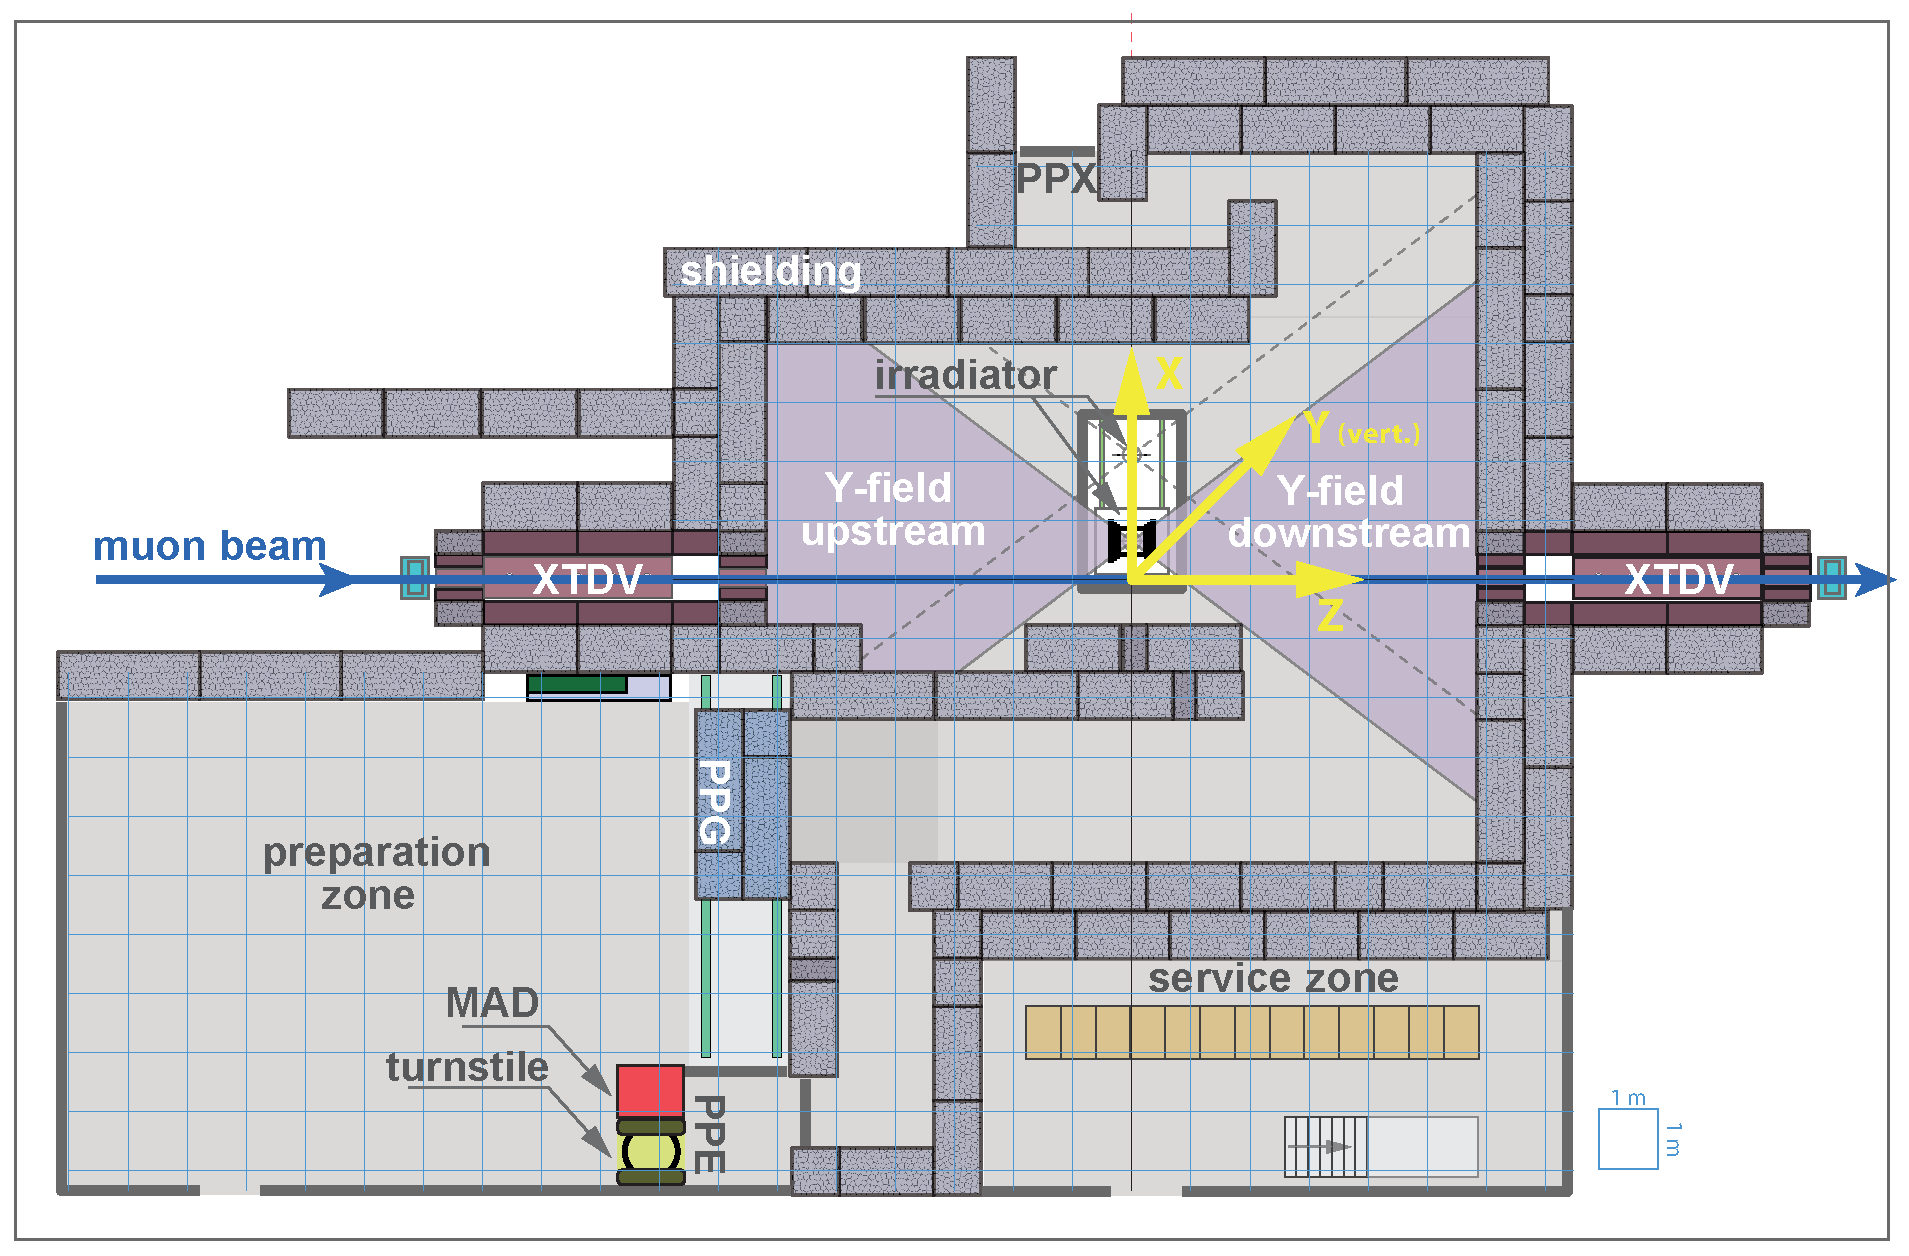
\includegraphics[scale=0.35]{fig/wincc/GIF.pdf}
  \caption{An overview of the GIF++ with entrance doors MAD (material access door), PPG (personal protection gate), PPE (personal protection entrance), PPX (personal protection exit).}
\label{fig:gif}
\end{figure}
The radiation field is uniformly distributed over the xy-plane as required for large-area flat detectors with the help of two $\pm \ang{37}$ angular correction filters both in the downstream and upstream regions. It is shown in Fig.~\ref{fig:attenuator_gif}a. The photon current is fine-tuned using two complete and independent attenuation systems. It consists of 3$\times$3 convex lead filters and attenuates photons that have energy less than 662\,keV to a higher degree. The attenuator system is shown in Fig.~\ref{fig:attenuator_gif}b with three planes (A, B, C) on either side of the source, and each plane further consists of three filters. Each filter possesses the nominal attenuation factors; 1 (A1,B1,C1), 1.5 (B2), 2.2 (C2), 4.6 (C3), 10 (A2), and 100 (A3, B3). A set of 24 nominal attenuation factors (nearly equidistant) have been selected from the 27 combination of 3$\times$3 that varies from 1 to 46415 as shown in Fig.~\ref{fig:attenuator_gif}c.  
\begin{figure}[htp]
\centering
\begin{tabular}{ccc}
\hspace{-0.2cm}
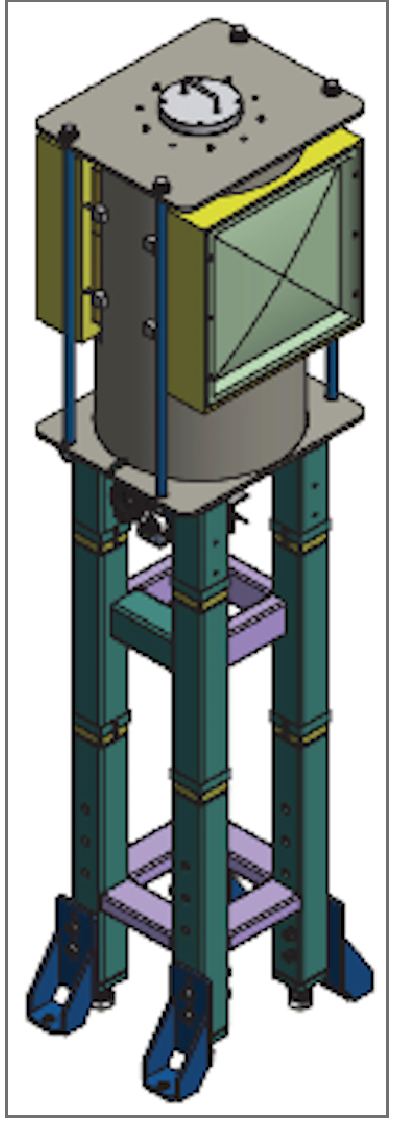
\includegraphics[scale=0.5]{fig/wincc/irradiator.pdf}
& \hspace{-0.632cm} 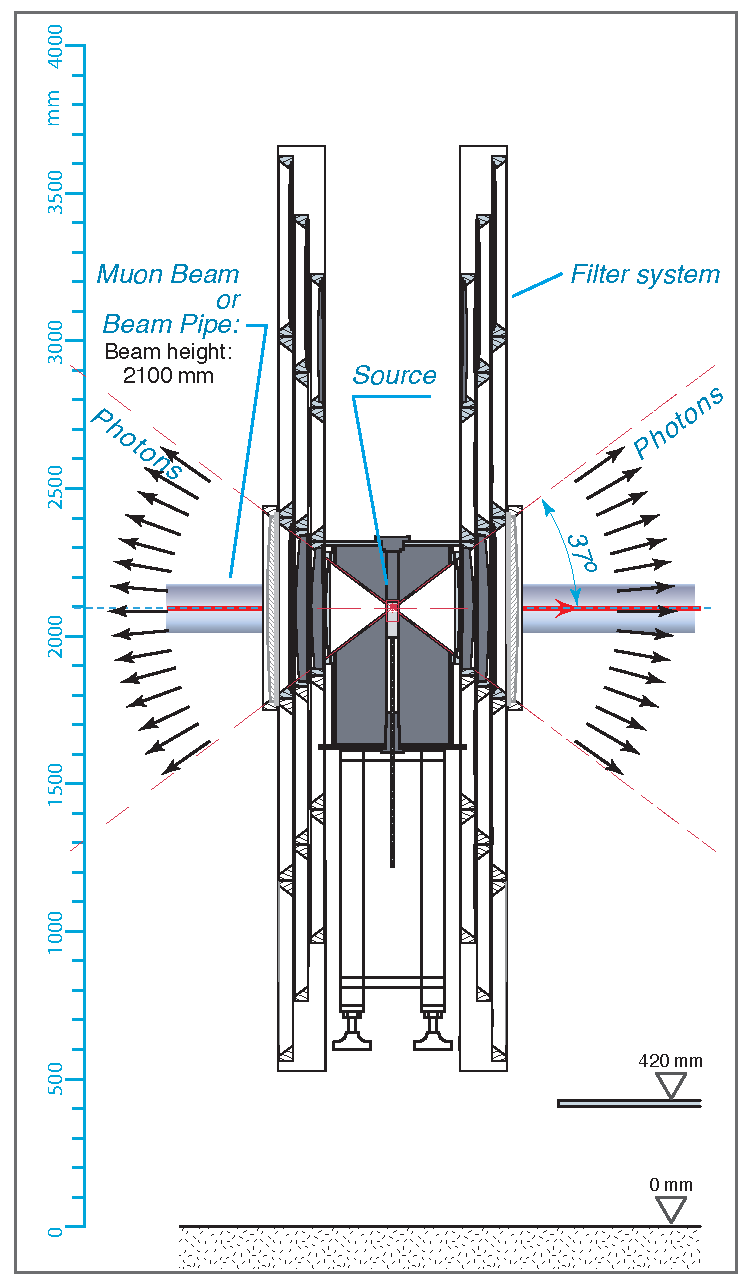
\includegraphics[scale=0.443]{fig/wincc/filters.pdf}
& \hspace{-0.65cm} 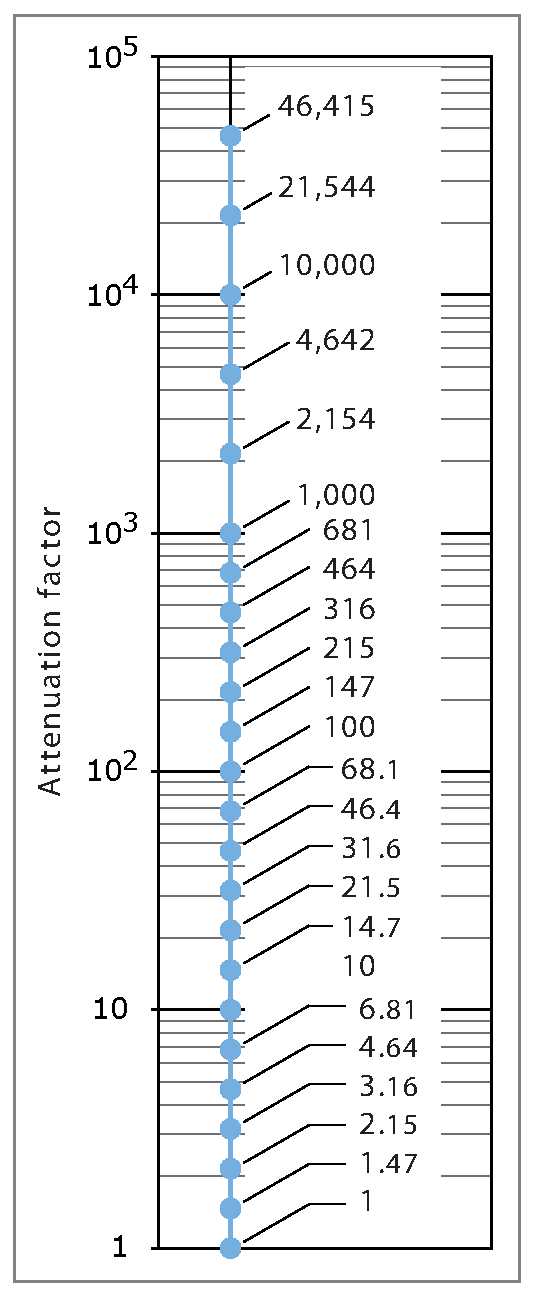
\includegraphics[scale=0.439]{fig/wincc/filter_factors.pdf}\\
  \qquad ($\mathbf{a}$)\qquad\qquad&($\mathbf{b}$)\qquad\qquad&($\mathbf{c}$)\\
\end{tabular}
\caption{Irradiator with the attenuator system in the GIF++. (a): Irradiator with independent angular correction filters on both sides. (b): Irradiator with remotely controlled attenuation filters to vary the radiation intensity. (c): A set of 24 nominal attenuation factors are selected from the 27 combination (3$\times$3) that varies from 1 to 46415.}\label{fig:attenuator_gif}
\end{figure}

Simulation of the 662\,keV photon current is shown in Fig.~\ref{fig:gif_simul} using an attenuator factor 1 (unattenuated). Using the angular correction filters, the current is uniformly distributed along the y-axis and varies from the source along the z-axis. 
\begin{figure}[h]
\centering
 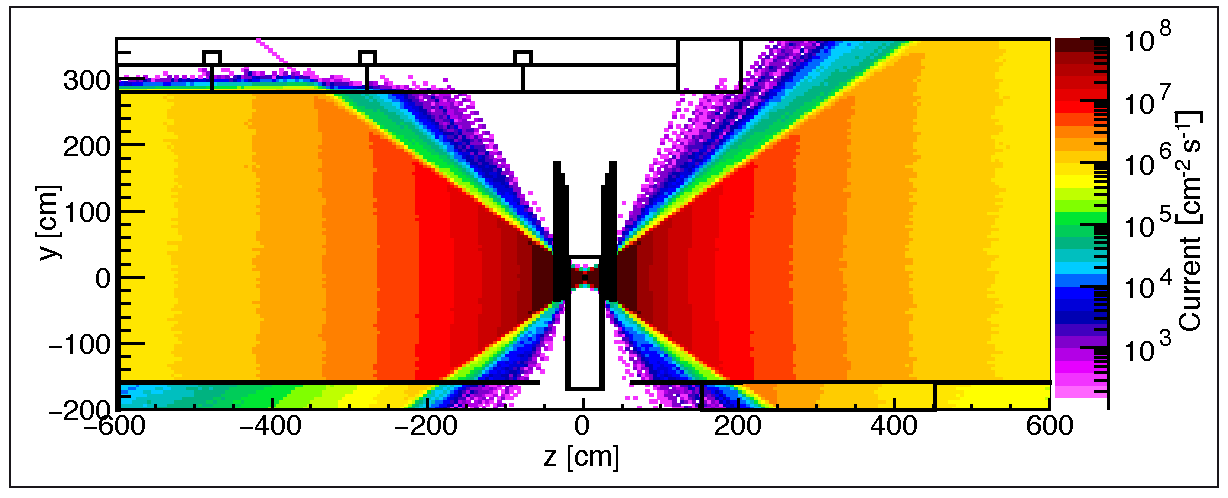
\includegraphics[scale=0.55,trim=0 0 0 0,clip]{fig/wincc/Current_gifpp_DS_US_flatSurfaceCurrent_600_662_x_60_70.pdf}
 \caption{Simulation of the unattenuated 662\,keV photon current in the yz-plane at x = 0.65\,m; using the angular correction filter.}
\label{fig:gif_simul}
\end{figure}

Table~\ref{tab:att_values} displays the nominal attenuation of 662\,keV photons and dose attenuation measured with the Automess gamma probe 6150AD-15 for different filter combinations. For factors less than 10, the nominal and effective dose attenuations are comparable while for greater than 10, the effective dose attenuation is considerably lower than the nominal attenuation factor, since scattered photons with an energy smaller than 662\,keV contribute substantially. 
\begin{table}[h]
\centering
\begin{tabular}{cc|c|c|}
\cline{3-4}
& & \multicolumn{2}{ c| }{Measured data} \\
\cline{1-4}
\multicolumn{1}{ |c|  }{Nominal} & Filter & Dose Rate & Dose \\
\multicolumn{1}{ |c|  }{Attenuation} & Combination & [mGy/h] & Attenuation \\ \cline{1-4}
\multicolumn{1}{ |c|  }{1 }      & A1 B1 C1 &   470.00   & -    \\ 
\multicolumn{1}{ |c|  }{1.5 }    & A1 B2 C1 &   400.00   & 1.2   \\
\multicolumn{1}{ |c|  }{2.2 }    & A1 B1 C2 &   211.00   & 2.2    \\
\multicolumn{1}{ |c|  }{4.6 }    & A1 B1 C3 &   105.00   & 4.5    \\
\multicolumn{1}{ |c|  }{10  }    & A2 B1 C1 &   55.00    & 8.8    \\
\multicolumn{1}{ |c|  }{100 }    & A3 B1 C1 &   6.50     & 72.3   \\
\multicolumn{1}{ |c|  }{100 }    & A1 B3 C1 &   6.20     & 75.8   \\
\multicolumn{1}{ |c|  }{464 }    & A1 B3 C3 &   1.59     & 295.6  \\
\multicolumn{1}{ |c|  }{4642}    & A2 B3 C3 &   0.22     & 2156.0 \\
\multicolumn{1}{ |c|  }{46415}   & A3 B3 C3 &   0.05     & 9400.0 \\ \cline{1-4}
\end{tabular}
  \caption{Nominal attenuation factors (attenuation of the 662\,keV photons) of some filter settings and measured effective attenuation in position D1 (x=0.65\,m, y=0.00\,m, z=1.10\,m)}
  \label{tab:att_values}
\end{table}

At the GIF++, the RPC detectors setup consists of two endcap chambers of type RE2 and RE4 that are continuously irradiated. Two non-irradiated chambers of the same type are installed to be used as reference. They are accompanied by the new generation of Glass-RPC (GRPC)~\cite{1748-0221-11-09-C09006} and multi-gap RPCs. A dedicated control system has been built to control these detectors and archive the relevant parameters using the WinCC-OA (PVSS) Supervisory Control And Data Acquisition (SCADA) system~\cite{twiki:wincc-oa}. The system controls high as well as low voltage supplies and monitors temperature, pressure, and humidity for both the RPC gas and the environment. The source status and attenuator values are accessed using the data interchange protocol (DIP), which is published centrally by the Engineering Department. The RPC gas supply is controlled and monitored by an external WinCC-OA project that shares relevant parameters with this project. All the relevant parameters are archived in a Structured Query Language (SQL) database (DB) for offline analysis.

One of the features of the GIF++ RPC DCS system is accessing the source status and attenuator values, as shown in Fig.~\ref{fig:attenuator_gif}c. Based on this information, the RPC performance parameters (efficiency, working point, cluster size, and resistivity) are measured. To retrieve the data from the database, a specific algorithm has been developed to synchronize the detector parameters (current and voltage) with the external parameters (temperature, pressure, and humidity). It enables the precise monitoring of the effect the external parameters have on the detector.
\section{WinCC-OA}\label{sec:wincc}
The SCADA System SIMATIC WinCC-OA~\cite{wincc_oa} is designed by ETM of the Siemens group and used extensively in large industries to supervise and control complex processes. Large experiments at CERN use the commercial ETM SCADA software, WinCC-OA, as a tool to develop control systems. WinCC-OA is consistently built on object-oriented structures, supported by both Windows and Linux systems, is flexible as well as distributed, and has an open architecture. 
WinCC-OA has the ability to connect hardware (or software) devices under a particular Detector Control System (DCS) and archive their data to observe the behaviour of the device under consideration. WinCC-OA describes a device in terms of a data point in a tree-like structure, with data point elements representing the device parameters. These can then be addressed directly to write to and read from the corresponding device. 
The WinCC-OA software runs different processes called ``Managers''. Event Manager (EV) is the heart of a WinCC-OA system, which connects other specific tasks managers. Figure~\ref{fig:wincc_managers} shows these managers and their specific functions. 
\begin{figure}[h]
\centering
 \includegraphics[scale=0.4,trim=0 0 0 0,clip]{fig/wincc/winccOA_manager.jpg}
 \caption{The concept of managers in WinCC-OA and it's functional layers. The event manager plays a key role in connecting all managers in a tree-like structure~\cite{wincc_managers}.}
\label{fig:wincc_managers}
\end{figure}

WinCC-OA is capable of building a distributed system in such a manner that different projects get interconnected and can exchange information remotely via the TCP/IP protocol using a ``Distribution'' Manager.
WinCC-OA uses a number of Managers as ``Drivers'' to communicate with the Front End (FE) hardware for data readout by mostly using the industry standard protocols, such as Profibus, CanBus, DIM, and Modbus, for communicating with the Programmable Logic Controllers (PLC) and OPC servers.
In order for non-experts to easily and safely operate the system, WinCC-OA provides a user-friendly Graphic User Interface (GUI) panel – an intuitive tool for controlling, monitoring, and operating the detectors in the safe mode. It provides the flexibility to combine text, graphical objects, and synoptic diagrams. The GUI panels can be used to observe the online behaviour of the detector in the form of plots, tables, and histograms. An example of the GUI is shown in Fig.~\ref{fig:gui}.
\begin{figure}[h]
\centering
\includegraphics[scale=0.5,trim=0 175 10 80,clip]{fig/wincc/GUI2.png}\\
 \caption{FSM main tree and high voltage scan panel using GUI.}
\label{fig:gui}
\end{figure}

All the LHC experiments have common tasks and requirements; therefore, it is necessary to have a general framework to provide all the required standard features and facilities. The Joint Controls Project (JCOP)~\cite{jcop} was developed to reduce the repetition of efforts by reusing common components and concealing the complexity of the underlying tools. The JCOP framework provides extra functions such as standardized Finite State Machine (FSM), the additional Graphical User Interface (GUI), the alarm handlers, and the ORACLE database interface~\cite{g-polese}.
The JCOP framework provides FSM toolkits in WinCC-OA based on State Machine Interface (SMI++). It offers an easy, robust, and safe way to control the full detector through the definition of a finite number of states, transitions, and actions (ON, OFF, STANDBY, Ramping Up, Ramping Down). A typical device state for an HV channel is implemented through the FSM mechanism, as shown in Fig.~\ref{fig:hierarchy}.
\begin{figure}[H]
\centering
\hspace{-0.5cm}
\includegraphics[scale=1.5,trim=160 600 160 120,clip]{fig/wincc/hierarchy.pdf}\\
 \caption{The DCS hierarchy tree for a typical high voltage channel using FSM. The tree shows a transition from one state to another.}
\label{fig:hierarchy}
\end{figure}
\section{The CMS RPC DCS project at GIF++}\label{sec:rpc_proj}
The CMS RPC DCS at GIF++ has been developed using WinCC-OA 3.11 and extended using the standard JCOP framework. It is designed in a tree-like structure with sub-systems of High Voltage (HV), Low Voltage (LV), environmental, and gas parameters (pressure, temperature, and humidity) as well as radiation levels. Each sub-system is mainly divided into two parts, the Front-End (FE) hardware located around the experimental area (sensors, power supplies, etc.) and a Back-End (BE) computer network wherein the DCS is running. The HV and LV power supplies used in the RPC GIF++ setup consist of CAEN SY1527 mainframe modules as well as CAEN EASY modules, with additional ADC modules used to read gas and environmental sensors (pressure, temperature, and humidity). The project has access to the hardware registered through Object Linking and Embedding (OLE) for Process Control (OPC) server provided by CAEN using the OPC protocol~\cite{opc}. The project controls the HV and LVsystem using the OPC protocol. The environmental and gas sensors (for pressure, temperature, and humidity) are also read out using the OPC protocol. The source status and attenuator values are available centrally via the DIP. The project has been designed to be distributed in order to enable communication with other projects and to read valuable information. Communication is established with the central GIF++ DCS in such a manner that the information from the gas system, such as flow rates, are readable.\\
The FSM hierarchy of the project is based on the naming convention of the trolley, where the detectors are installed. Each trolley has six sections and each section accommodates one detector. Currently, three CMS RPCs trolleys are installed in the GIF++. Trolley~1 (RPC Consolidation) is equipped with spare RPCs, trolley~2 with small glass RPCs, and trolley~3 with prototypes of improved RPCs. Figure~\ref{fig:rpc_setup} shows the RPCs configuration in a trolley, and detailed information of the trolleys are provided here~\cite{salvador}. 
A schematic overview of the DCS project is shown in Fig.~\ref{fig:DCS_sys}.
\begin{figure}[h]
\centering
\includegraphics[scale=0.4,trim=60 30 60 30,clip]{fig/wincc/DCS_sys.png}\\
 \caption{An overview of the CMS RPC DCS at the GIF++.}
\label{fig:DCS_sys}
\end{figure}
\subsection{High and low voltage system}
The power supply system provided both HV and LV to the installed RPCs in the GIF++. Owing to the simple setup, both the HV and LV boards were installed in the CAEN mainframe that are located outside the radiation zone.
The high and low voltage system is controlled and monitored by the CAEN OPC server. Each gap in a chamber is independently connected to a single high-voltage channel, which improves the granularity of control. The RPC front-end electronics requires digital and analogue power supplies~\cite{feb}. Each low-voltage line has been shared between the two front-end-boards (FEBs) for digital as well as for analogue power supply. The DCS communication with the CAEN mainframe is shown in Fig.~\ref{fig:caen_control}
\begin{figure}[h]
\centering
\includegraphics[scale=1.0,trim=60 380 60 320,clip]{fig/wincc/caen_control.pdf}\\
 \caption{The HV and LV channels can be operated by the CAEN mainframe independently, and the DCS is connected to the CAEN via OPC server. An easy crate is used for environmental and gas parameter measurement.}
\label{fig:caen_control}
\end{figure}
\subsection{Environmental and gas parameters}
The performance of the RPCs strongly depends on the temperature and pressure of the environment because the RPC's gas density is directly affected by these parameters. Hence, it is important to measure the environmental parameters (temperature, pressure, and humidity) at different locations where the RPCs are installed. The applied voltage is corrected for the environmental temperature and pressure in order to include their effects using Eq.~\ref{equ:temp_press_correc}:  
\begin{equation}\label{equ:temp_press_correc}
HV_{app}(P, T) = HV_o . \frac{P_o}{P}\frac{T}{T_o}
\end{equation} 
Where $P_o$, $T_o$ are the environmental and $P$, $T$ are the bunker (the radiation zone) pressures and temperatures respectively. $HV_o$ is the user set-up high-voltage and $HV_{app}$ is the corrected high voltage supplied by the DCS system.
This procedure is described in detail in~\cite{env-rpc}. 
Figure~\ref{scan_temp}a provides a plot for the environmental temperature, pressure, and humidity. The environmental and gas sensors (temperature, pressure and humidity) are readable through the ADC (analog-to-digital converter) board that is installed in the EASY crate. The JCOP framework presents the opportunity to convert the ADC counts into physical values online. The trending feature provides a comparison between different sensors located at different positions.
\subsection{High voltage scan and stability test}
The project has been designed for the R\&D of detectors. Hence, it should be able to perform high-voltage scanning or stability tests. For high-voltage scanning, a separate branch has been incorporated in the FSM tree, wherein the user operates each detector independently. 
A typical UI panel used for HV scanning is shown in Fig.~\ref{fig:gui}(right). Using this panel, a user can select different voltage values (left column), a single current value (second left column), and operate detectors independently (third column). The user has access to mask a single HV channel (connected to a specific part of the RPC detector) without making the whole detector. 
The stability test runs for a long period of time in order to expose the detectors to high radiation. Based on the requirements, a dedicated manager applies the stability script and restarts it automatically. An example of a HV scanning plot for one of the CMS RPC chambers (RE3) at GIF++ is shown in Fig.~\ref{scan_temp}b. 

\begin{figure}[h]
\centering
\begin{tabular}{cc}
\hspace{-0.3cm}
\includegraphics[scale=0.33,trim=50 70 20 90,clip]{fig/wincc/tprh.png}
& \hspace{-0.5cm} \includegraphics[scale=0.345,trim=50 100 45 80,clip]{fig/wincc/HV_Scan2.png}\\
   ($\mathbf{a}$)\qquad&($\mathbf{b}$)\qquad\\
\end{tabular}
\caption{(a): Environmental temperature ($^o$C), pressure (mb), and humidity (\%). Time is on the x-axis while the red, blue, and green lines represent the values of pressure, temperature, and humidity respectively on the y-axis. The pressure and temperature values used for operating voltage correction of the RPCs. (b): A HV scan of the CMS RE3 chamber. The x-axis shows time while the y-axis shows the voltage (V) and current ($\mu$A) values. The red, blue, and green lines are voltages while the cyan, brown, and orange lines are the corresponding current values for bottom, top-narrow, and top-wide gaps respectively.}\label{scan_temp}
\end{figure}

\subsection{Database}
To study the behaviour of the detector over time and to perform an offline data analysis, it is necessary to store all the important parameters in a database. In particular, the HV, LV, environmental and gas parameters, and radiation levels (attenuator values) are kept for this purpose. This information can be utilized to constantly check the online behaviour of a detector during operation and for the offline analysis to measure the ageing effects after it has absorbed a specific radiation dose. WinCC-OA's uses an internal database for small and simple projects, which stores data locally on the hard drive or on an external oracle database for more complex technical processes that generate large quantities of data. The Relational Database Manager (RDB) is specifically assigned to archiving data in the external oracle database. 

Compared to the central CMS RPC system, the RPCs at the GIF++ generate a small amount of data; hence, we used the internal built-in SQL database in this project. It doesn't need the RDB manager to run. The data point is archived in the database when a change occurs in its value. To suppress the noise fluctuation and reduce the size of data, a ``deadband'' is specified for each archiving parameter. Since the changes in environmental parameters and HV don't occur at the same time, the values stored in the database are not synchronized. A specific algorithm is applied to synchronise all the relevant stored parameters for analysis. The stored data is finally extracted to be used for the offline analysis using a GUI.


\section{CMS RPC longevity studies}
RPCs are gaseous detectors and in principle can suffer from ageing effects when exposed to a prolonged radiation that deteriorates the detector performance in the form of efficiency loss, dark rate, dark current etc. The deterioration is mainly caused by complicated chemical processes largely occurring in the hot plasma inside electron multiplication avalanches where gas molecules may form polymers growing on electrodes. The severity of ageing increases with integral of radiation exposure and depends on a myriad of factors, such as detector geometry, the materials used for the electrodes, operational gas gain, gas mixture, impurities in the gas itself, gas flow rate etc. 
For the life span of an experiment, the ageing effects of the installed detectors can be studied by subjecting the same detectors prototypes to accelerated ageing tests performed at a higher instantaneous radiation rate. Assuming the dependency of detector's ageing on the accumulated charge per unit area (in case of RPC), the obtained results from these tests can be projected towards many years of operation at the expected nominal radiation. Since this is approximation and quantitatively not productive, so a large safety margin factor of 3 is used to accumulate the total amount of radiation precisely. The performance of the installed CMS RPC system has already been certified for 10~LHC years in the GIF facility at maximum background rate of 300\,Hz-cm$^{-2}$ and a total integrated charge of 50\,mC-cm$^{-2}$~\cite{ABBRESCIA2004102}.

The background rates showed linearly dependency on the instantaneous luminosity during the Run-I and Run-II data taking periods both in barrel as well as in endcap regions. Assuming the same linear relationship, the expected rates are extrapolated to the HL-LHC conditions reaching up to 600\,Hz-cm$^{-2}$ including a safety factor of 3, as shown in Fig.~\ref{fig:cms_rpc_extrapolated_rates} for all barrel (left) and endcap (right) chambers. Using the same safety factor, the expected integrated charge in the hottest region of the current RPC system will be 840\,mC-cm$^{-2}$ at the end of the HL-LHC. The same amount of integrated charge will be accumulated in the GIF++ facility to certify the detectors for HL-LHC conditions. 
  
\begin{figure}[h]
\centering
\includegraphics[width=0.49\textwidth,keepaspectratio=true]{fig/wincc/longevity/Barrel-Roll-Rate-HL-LHC.pdf}
\includegraphics[width=0.49\textwidth,keepaspectratio=true]{fig/wincc/longevity/Endcap-Disks-Rate-HL-LHC.pdf}
\caption{Extrapolation from 2016 data of single hit rate per unit area to HL-LHC conditions, in the barrel (left) and endcap (right) regions, for the present RPC system.}
\label{fig:cms_rpc_extrapolated_rates}
\end{figure}

The longevity study has already been started in the GIF++ facility by continuously irradiating the two turned on chambers, RE2/2 and RE4/2. The total integrated charge accumulated by the two chambers are shown in Fig.~\ref{fig:gifpp_integrated_Q}. At the end of 2017, the total integrated charge for RE2/2 and RE4/2 was about 292\,mC-cm$^{-2}$ and 119\,mC-cm$^{-2}$ respectively which corresponds to 34\% and 14\% of the expected integrated charge at the HL-LHC. Due to gas flow limitation, the RE4/2 was turned on later.   
\begin{figure}[h]
\centering
\includegraphics[width=0.59\textwidth,keepaspectratio=true]{fig/wincc/longevity/GIFPP_Integrated_Charge.pdf}
\caption{Integrated charge versus time accumulated during the GIF++ studies for the RE2/2 (red) and RE4/2 (blue) chambers. Because of total gas flow limitations, the RE4/2 chamber has been turned on few months later. Different slopes account for different irradiation conditions during data taking.}
\label{fig:gifpp_integrated_Q}
\end{figure}

\subsection{RPCs setup at GIF++ for efficiency studies}\label{eff_calc}
Four RPC chambers (two RE2 and two RE4~\cite{feb}) are placed parallel to each other in a vertical position, a few meters away from the source in the upstream area as shown in Fig.~\ref{fig:rpc_setup}.
\begin{figure}[h]
\centering
\includegraphics[scale=0.07]{fig/wincc/RPC_setup.jpg}\\
 \caption{CMS RPCs setup in the GIF++. Detectors are placed perpendicularly and a few meters away from the source.}
\label{fig:rpc_setup}
\end{figure}
Several high-voltage scans were performed using different radiation levels (starting from the absence of radiation source) to define the optimal operating voltage of each chamber, which is called Working Point (WP). The efficiency (E) for different background radiation levels is calculated using the equation:
\begin{equation}
 {E = N_{RPC}/N_{TRACK}.}
\end{equation}
The muon track is reconstructed using three reference RPC planes and extrapolated to the RPC under test, examining the closest cluster (a strip or set of continuous strips). N$_{TRACK}$ corresponds to the number of muons passing through the three reference RPC detectors at the same time. N$_{RPC}$ corresponds to the number of fired clusters in the chamber under test. The dependence of the efficiency E on the effective high voltage HV$_{eff}$~\cite{hv-eff} can be fitted using the following sigmoidal curve:
\begin{equation}
{\langle E\rangle = E_{max} / (1 + exp (-\lambda (HV_{eff} - HV_{50\%})),}
\end{equation}
where E$_{max}$ is the maximum efficiency reached by the chambers at HV$\rightarrow \infty$, $\lambda$ is proportional to the slope of sigmoid at flex point, and HV$_{50\%}$ is the high voltage at which a chamber reaches 50\% of its maximum efficiency. The Working Point of a chamber is defined by:
\begin{equation}
 HV_{wp} = HV_{knee} + 150V,
\end{equation} 
where HV$_{knee}$ is the voltage at which the efficiency is 95\% of the maximal one.   

\subsection{Efficiency and cluster size results}
In Fig.~\ref{eff}a, the efficiency as a function of HV$_{eff}$ for different radiation levels is presented. The maximum efficiency slightly decreases with the amount of radiation received by the detector. In Fig.~\ref{eff}b, the maximum efficiency as a function of the gamma hits rate is presented for four RPC chambers. The RPCs were placed parallel to each other, with RPC-1 being the closest to the source while RPC-4 was the furthest. The radiation dose depends on the distance between the RPCs and the gamma source. RPCs 3 and 4 received a smaller dose as compared to RPCs 1 and 2. 
\begin{figure}[h]
\centering
\begin{tabular}{cc}
\hspace{-0.5cm}
\includegraphics[scale=0.30,trim=0 13 0 0,clip]{fig/wincc/eff.png}
& \hspace{-0.60cm} \includegraphics[scale=0.329,trim=0 0 0 0,clip]{fig/wincc/rate_eff.png}\\
   ($\mathbf{a}$)\qquad&($\mathbf{b}$)\qquad\\
\end{tabular}
\caption{(a): Efficiency vs HV$_{eff}$ for different gamma attenuator factors. (b): Maximum efficiency vs gamma rate at HV$_{wp}$ for four RPCs.}\label{eff}
\end{figure}

Figure.~\ref{eff} represents the very first results obtained in the GIF++ at the start of 2016. Afterwards, several measurements have been performed under different background radiation conditions using the dedicated attenuator system. Each time the detector performance has been studied. Figure~\ref{fig:cms_rpc_eff_diff_periods} shows the hit efficiency of the RE2/2 chamber as a function of the effective HV at different irradiation stages, corresponding to an integrated charge of 0, 153\,mC-cm$^{-2}$ and 257\,mC-cm$^{-2}$. The background radiation rate is minimum (source-off) in the left plot and maximum (about 600\,Hz-cm${-2}$) in the right plot. The detector showed stable behaviour over time and no change in the efficiency and working point has been observed.    

\begin{figure}[h]
\centering
\includegraphics[width=0.49\textwidth,keepaspectratio=true]{fig/wincc/longevity/RE2-Efficiency.pdf}
\includegraphics[width=0.49\textwidth,keepaspectratio=true]{fig/wincc/longevity/RE2-Efficiency-600.pdf}
\caption{Hit efficiency of RE2/2 as a function of the effective HV, without irradiation (left) and under a gamma background rate of about 600\,Hz-cm$^{-2}$ (right). The measured efficiency of the RE2/2 chamber corresponds to different Test Beams (TB) with integrated charge: 0, 153\,mC-cm$^{-2}$ (18\%) and 257\,mC-cm$^{-2}$ (31\%). The detector performance is stable at high fraction of accumulated charge.}
\label{fig:cms_rpc_eff_diff_periods}
\end{figure}

A similar study has been done to monitor the cluster size, defined as the number of fired strips per hit. Figure~\ref{fig:cms_rpc_cluster_diff_periods} shows the cluster size as a function of effective HV for RE2/2 chamber with integrated charge: 153\,mC-cm$^{-2}$ (18\%) and 257\,mC-cm$^{-2}$ (31\%) without background radiations (left) and background gamma irradiation of about 600\,Hz-cm$^{-2}$ (right). No significant change has been observed in the cluster size.

\begin{figure}[h]
\centering
\includegraphics[width=0.49\textwidth,keepaspectratio=true]{fig/wincc/longevity/RE2-ClusterSize.pdf}
\includegraphics[width=0.49\textwidth,keepaspectratio=true]{fig/wincc/longevity/RE2-ClusterSize-600.pdf}
\caption{Cluster size of RE2/2 as a function of the effective HV, without irradiation (left) and under a gamma background rate of about 600\,Hz-cm$^{-2}$ (right). The measured cluster size of the RE2/2 chamber corresponds to different Test Beams (TB) with integrated charge: 153\,mC-cm$^{-2}$ (18\%) and 257\,mC-cm$^{-2}$ (31\%). The cluster size is above 2 at working point of the detector with high fraction of accumulated charge.}
\label{fig:cms_rpc_cluster_diff_periods}
\end{figure}

\section{Summary} 
The DCS project for the CMS RPCs has successfully been implemented and tested in the CERN GIF++. Since June 2015, the project has been running in a stable manner. The detectors are being operated and the data being archived. The hardware integrated in the project fully controls the high-voltage scanning and stability tests. Environmental and gas sensors are included and used for temperature and pressure corrections. Gas flow-meters are read through the central DCS at GIF++, and the data is used to study the behaviour of different gas mixtures. All useful parameters are archived in the internal database for offline analysis. As the project is designed for detector R\&D studies, any new hardware can be added easily and safely.

The performance of the CMS RPC chambers at GIF++ has been studied and compared at different radiation levels. At a rate of 600\,Hz-cm$^{-2}$, the Eff$_{max}$ of the chamber was 95\%. 
The detectors showed stable performance up to 34\% of the expected integrated charge that will be accumulated at the end of the HL-LHC run. 
%\acknowledgments We wish to congratulate our colleagues in the CERN Engineering- (EN) and Physics- Department (PH) for successful operation of the GIF++. We thank the technical and administrative staff at CERN, other CMS institutes and RPC group. Many thanks to ATLAS colleague Marino Romano for his technical support to develop the project.   



%\renewcommand*{\thesection}{\thechapter.\arabic{section}}       % reset again to chaptnum.sectnum

%\clearpage{\pagestyle{empty}\cleardoublepage}
